Con el surgimiento del computador y su capacidad de poder realizar gran cantidad de c�lculos de manera eficiente se abrieron un sinn�mero de posibilidades. Lo que antes era hecho manualmente por personas, ahora es superado en tiempo y exactitud por una m�quina.
Esta capacidad ha sido explotada con diversos fines, entre los cuales podemos mencionar como ejemplos el procesamiento de texto, gr�ficos y c�lculos matem�ticos. Con la aparici�n de nuevas aplicaciones de software cada vez m�s exigentes en recursos computacionales, los requerimientos de procesamiento han ido en aumento lo que implica cada vez nuevos desaf�os para la computaci�n.
Para satisfacer esta demanda, se han propuesto diversas soluciones. Desde el punto de vista de la industria del hardware se pueden distinguir dos tendencias. Una de ellas apunta a la mejora de los componentes del hardware como procesadores, co-procesadores, memorias y otros dispositivos de hardware especializados. La otra corriente apunta a ofrecer grandes sistemas de c�mputo dedicados, llamados \emph{clusters}, que no son m�s que aglomeraciones de computadores coordinados entre s� para aparecer frente al usuario como una poderosa unidad de procesamiento.

Actualmente en algunas disciplinas como las ciencias existen grandes necesidades de c�mputo y frecuentemente se opta por adquirir clusters para satisfacer aquellas demandas. Si bien esta soluci�n es natural y ampliamente usada, tiene un gran inconveniente: su elevado costo. Adem�s considerando que la rapidez del desarrollo de hardware deval�a r�pidamente lo adquirido, hace que tal inversi�n parezca tener menos fundamento para organizaciones cuyos presupuestos se mantienen siempre restringidos.

En la actualidad los computadores personales est�n en todas partes, en hogares, oficinas y laboratorios entre otros. Si bien estas m�quinas representan una herramienta para sus due�os y usuarios, considerando su potencial desde sus especificaciones hardware, se puede llegar f�cilmente a la conclusi�n de que generalmente est�n siendo subutilizadas durante una cantidad de tiempo considerable. Sin ir m�s lejos, en muchos laboratorios de computaci�n jam�s se apagan los computadores y cuando se encuentran cerrados por las noches se encuentran todos ellos ociosos, lo que representa un gran potencial de c�mputo perdido.
Existiendo una demanda de procesamiento y por otra parte, tiempo de procesamiento no utilizado, s�lo falta el mecanismo que re�na ambas partes y logre trasformar este potencial en trabajo �til. El presente proyecto tiene como fin desarrollar un sistema que represente tal mecanismo. Sin embargo, como se expone en la siguiente secci�n de este mismo cap�tulo\footnote{Secci�n \ref{ref:intro_motivacion}}, la creaci�n de tal sistema tiene una serie de problemas y desaf�os subyacentes que trascienden a lo netamente t�cnico e inf�rmatico, y hace necesario considerar la dimensi�n social de �ste. Tales aspectos est�n impl�citos en los objetivos del presente proyecto presentados en la secci�n de descripci�n de este mismo cap�tulo\footnote{Secci�n \ref{ref:intro_descripcion}}.
\section{Motivaci�n}\label{ref:intro_motivacion}
Actualmente en el \emph{PROFC}\cite{profcpage} (Laboratorio de Procesos Oceanogr�ficos y Clima)\footnote{En realidad la sigla significa \emph{Programa Regional de Oceanograf�a F�sica y Clima}, nombre del programa original que finalmente se consolid� con el nombre actual} de la Universidad de Concepci�n, sus investigadores recurren a diversos programas utilitarios que son esenciales para el desarrollo de sus tareas. Muchas de estas aplicaciones se caracterizan por el alto tiempo de c�mputo que requieren en relaci�n al tama�o de la entrada de datos. Generalmente las tareas que se procesan son un gran n�mero de ejecuciones de un mismo programa con diferentes entradas. Si se ejecutara tal tarea de una manera serializada, entonces el tiempo que transcurra desde su inicio hasta su t�rmino puede tener una duraci�n no aceptable.

Teniendo en cuenta la gran cantidad de computadores que se encuentran conectados a la red institucional, en su mayor�a en laboratorios, y que existen per�odos de tiempo en que no son utilizados intensamente, como en las noches, fines de semanas, feriados y per�odos de vacaciones, entonces se podr�a implementar un sistema que permita distribuir una tarea en todos estos computadores ociosos con el fin de reducir el tiempo de ejecuci�n de estas.
Ante el usuario, el sistema se comportar�a como una poderosa m�quina, un cluster virtual al que se le asignan tareas a ejecutar. No obstante para llevar a cabo la idea hay que considerar los siguiente aspectos :
Los computadores que conforman el cluster virtual ya poseen una funci�n primaria. Por ejemplo, un computador de laboratorio tiene como funci�n primaria ser una herramienta para un usuario que disponga de �l. Si bien se pretende que el cluster virtual haga uso de este computador, no debe ser en perjuicio de su funci�n primaria, ya que no son m�quinas dedicadas. En otras palabras, el sistema debe ser invisible ante el usuario que ocupe dicha m�quina. El cluster virtual debe ser capaz de detectar cu�ndo una m�quina se encuentra disponible para su uso y cu�ndo no.

El cluster virtual tendr� la caracter�stica de que entre m�s computadores lo compongan, m�s poderoso ser� y m�s eficientemente puede responder a las demandas de los usuarios. Por eso es de suma importancia que el sistema est� dise�ado para incluir la mayor cantidad de m�quinas. Esto se traduce en que, aspectos como los diferentes sistemas operativos instalados en los computadores, y las estructuras de red en las cuales se encuentran, no deben ser un impedimento para agregar un computador al sistema.

Otro desaf�o subyace al ideal de instaurar el cluster virtual de manera institucional en la red de la Universidad de Concepci�n. Si bien el cluster virtual representa un beneficio para sus usuarios, no es tan claro el beneficio que recibir�a la instituci�n, m�s a�n si se van a usar recursos de �sta. Debido a esto, una funci�n secundaria que reporte un beneficio para la Universidad se convierte en un aspecto importante. Ante la carencia de la Universidad de poseer un salvapantallas institucional y aprovechando que el sistema llegar�a a todos los computadores usados por la comunidad universitaria, dotar al sistema de un salvapantallas que sirva como medio de comunicaci�n, de modo que �ste despliegue informaci�n relevante sobre la comunidad Universitaria, como noticias, se convertir�a en una funcionalidad que reportar�a beneficios para la instituci�n, lo que ayudar�a a lograr lo inicialmente mencionado, instaurar el cluster virtual institucionalmente.
\section{Descripci�n del proyecto}\label{ref:intro_descripcion}
El objetivo principal del proyecto es desarrollar e implementar un sistema que permita aprovechar el tiempo ocioso de computadores para realizar procesos definidos por usuarios, tal como se muestra en la figura \ref{fig:image03}.
El perfil de los computadores objetivos son m�quinas que se encuentran mucho tiempo siendo no utilizadas, como las m�quinas dentro de un laboratorio de computaci�n, que generalmente est�n encendidas sin que ning�n usuario las ocupe.
Esto excluye a notebooks u otros computadores port�tiles dado que, por su naturaleza m�vil, hace que no cumplan el perfil anteriormente expuesto dado que si un notebook no se est� usando, generalmente el usuario tiende a apagarlos. Los computadores de laboratorio por lo general cuentan con un sistema operativo basado en Windows XP o Linux, por esta raz�n el sistema debe ser compatible con ambas plataformas.
Los procesos definidos por el usuario corresponden a un conjunto de ejecuciones de un programa de l�nea de comandos. La ejecuci�n del programa conforma la unidad b�sica de procesamiento dentro del sistema. Este hecho determina el nivel de paralelismo que maneja el sistema, que consta en correr varios procesos simult�neamente.
El sistema debe estar enfocado en el procesamiento de grandes vol�menes de datos, lo que quiere decir que los usuarios del sistema pueden ejecutar en �l una cantidad de procesos del orden de los cientos de miles.
El segundo objetivo es proveer al sistema de una plataforma de comunicaci�n en la forma de un salvapantallas que est� en cada computador que conforma el sistema. Esta plataforma de comunicaci�n consiste en que usuarios con privilegios especiales pueden establecer conjuntos de p�ginas web para ser desplegadas c�clicamente por los salvapantallas de cada computador perteneciente a grupos determinados. Por ejemplo, las p�ginas pueden ser sitios institucionales que contengan noticias y avisos �tiles para personas que frecuentan dichos computadores.
\begin{figure}
\begin{center}
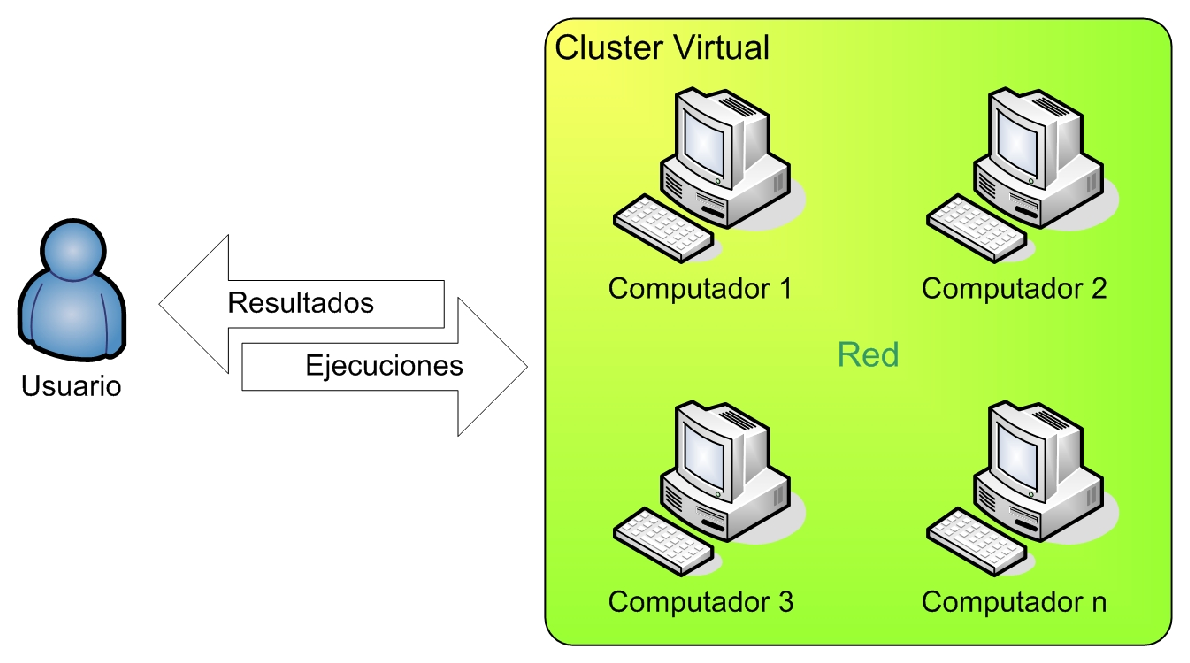
\includegraphics[width=0.7\textwidth]{images/image03.eps}
\end{center}
\caption{Esquema del sistema de cluster virtual}
\label{fig:image03}
\end{figure}
Para alcanzar los objetivos antes descritos se debe alcanzar una serie de etapas que comprenden los objetivos espec�ficos del proyecto. Los objetivos espec�ficos agrupados en sus respectivas etapas se describen a continuaci�n:
\paragraph{An�lisis bibliogr�fico}
Esta etapa consiste en un estudio sobre el tema de la computaci�n distribuida. Los objetivos de esta etapa son obtener antecedentes generales sobre el contexto del proyecto, describir los requerimientos del sistema y los recursos disponibles que hacen factible su implementaci�n, y analizar algunas de las soluciones existentes para establecer un punto base para el establecimiento de la arquitectura del proyecto.
\paragraph{Dise�o}
El objetivo de esta etapa es traducir los objetivos del proyecto en el dise�o de una soluci�n, en espec�fico, la arquitectura del sistema. En esta etapa se deben tratar los problemas l�gicos que surgen y las metodolog�as que permiten solucionarlos. 
\paragraph{Implementaci�n}
El objetivo de esta etapa es implementar la arquitectura del sistema en un software funcional. En esta etapa se deben tratar los problemas inherentes a la implementaci�n y la forma en que se abordan para darles soluci�n.
\paragraph{Evaluaci�n}
Los objetivos de esta etapa consisten en crear una aplicaci�n que utilice el sistema de cluster virtual y evaluar el rendimiento de �ste.

\section{Estructura del documento}
El desarrollo del presente informe se estructura en seis cap�tulos.

En el cap�tulo \ref{ref:chapter_antecedentes} se presentan antecedentes generales sobre el tema de la computaci�n distribu�da haciendo especial hincapi� en el an�lisis de dos soluciones existentes. Adem�s se describen los requerimientos y la factibilidad del sistema.

El cap�tulo \ref{ref:chapter_arquitectura} tiene como objetivo definir l�gicamente la soluci�n, estudiando aspectos como la arquitectura y funcionamiento del sistema.

En el cap�tulo \ref{ref:chapter_implementacion} se tratan los temas respectivos a la implementaci�n de la soluci�n, tales como las tecnolog�as a utilizar, la estructura interna de las piezas de software y metodolog�as utilizadas.

En el cap�tulo \ref{ref:chapter_comunicacion} se describen los aspectos relativos a la comunicaci�n de los diferentes elementos de software que componen el sistema. Se detallan los protocolos de comunicaci�n usados as� como tambi�n las soluciones a diversos problemas inherentes al uso de �stos.

En el cap�tulo \ref{ref:chapter_evaluacion} se presenta la aplicaci�n de prueba, donde se implementa el sistema para su evaluaci�n. Tambi�n son mostrados los resultados de las pruebas con sus respectivos an�lisis.

Finalmente, en el cap�tulo \ref{ref:chapter_conclusiones} se presentan las conclusiones extra�das del proceso de desarrollo del proyecto.

Adicionalmente hay una secci�n de anexos al final del documento, donde fueron relegados los desarrollos demasiado extensos o de naturaleza demasiado espec�fica que son referenciados a lo largo del documento.